%%%  default
\documentclass[10pt, compress]{beamer}


\usetheme{mnuigD}
\usepackage{tikz}
\usepackage{booktabs}
%\usepackage{cite}
\bibliographystyle{apalike}
\usepackage[export]{adjustbox}
\usepackage{subfig}
\usepackage[export]{adjustbox}
% \usepackage[scale=2]{ccicons}
\usepackage[normalem]{ulem} % for strikethorugh
%\usemintedstyle{trac}
\usepackage{grffile} %for underscores in file names
\title{Collaboration in the 21\textsuperscript{st} century:\\ tips and tools for dealing with data}
\subtitle{{\small (or, how I learned to stop worrying and love version control)}}
% \subtitle{NUIG Bioinformatics}
\date{\footnotesize{ Hot Topic: \today}}
\author{
  % \vspace{10mm}
  % \hspace{5mm}
\includegraphics[height=30mm]{./20170202_bss_figs/logo_1_dark}
\\ \\ \\ \\ \large{Nick Waters}}
\institute{
National University of Ireland, Galway\\
James Hutton Institute, Dundee}

%%%%% %%%%% %%%%% %%% %%%%  for pretty headers with pictures
\addtobeamertemplate{frametitle}{}{%
\begin{tikzpicture}[remember picture,overlay]
\node[anchor=north east,yshift=2pt] at (current page.north east) {
\includegraphics[height=0.8cm]{../stock_logos/nuig_rounded.png}  \hspace*{.05cm} 
\includegraphics[height=.794cm, trim= 0cm 0.0cm 0.0cm 0cm]{../stock_logos/jhi_rounded.png}};
\end{tikzpicture}}


\begin{document}
\maketitle

%\maketitle
\setbeamertemplate{itemize items}[square]
\section{The Problem: other people's data}

\section{The Problem: my data}

\begin{frame}[fragile]
  \frametitle{Bad Data}
  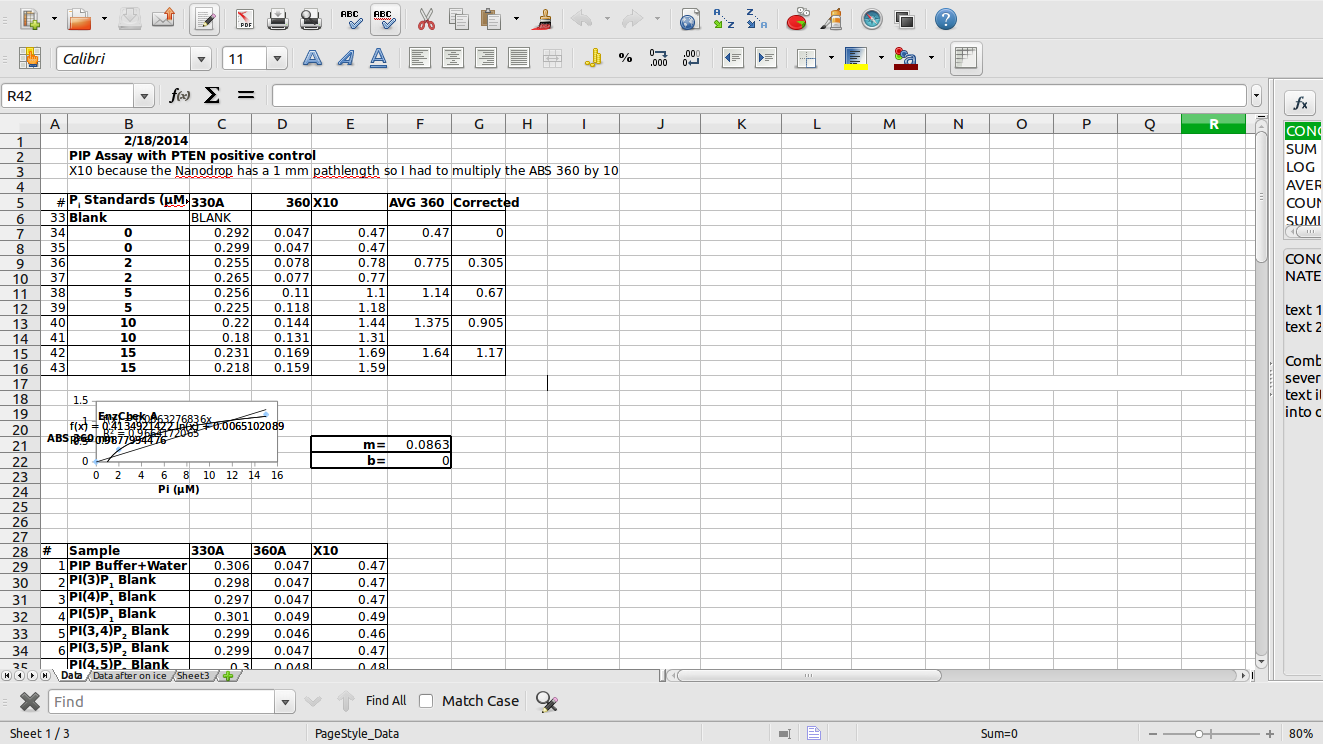
\includegraphics[width=.99\textwidth]{~/GitHub/FB/Ecoli_comparative_genomics/doc/presentations/MyNUIG(mnuigtheme)/20170303_ht_figs/pip_assay.png}
\end{frame}

\begin{frame}[fragile]
  \frametitle{Bad Data}
  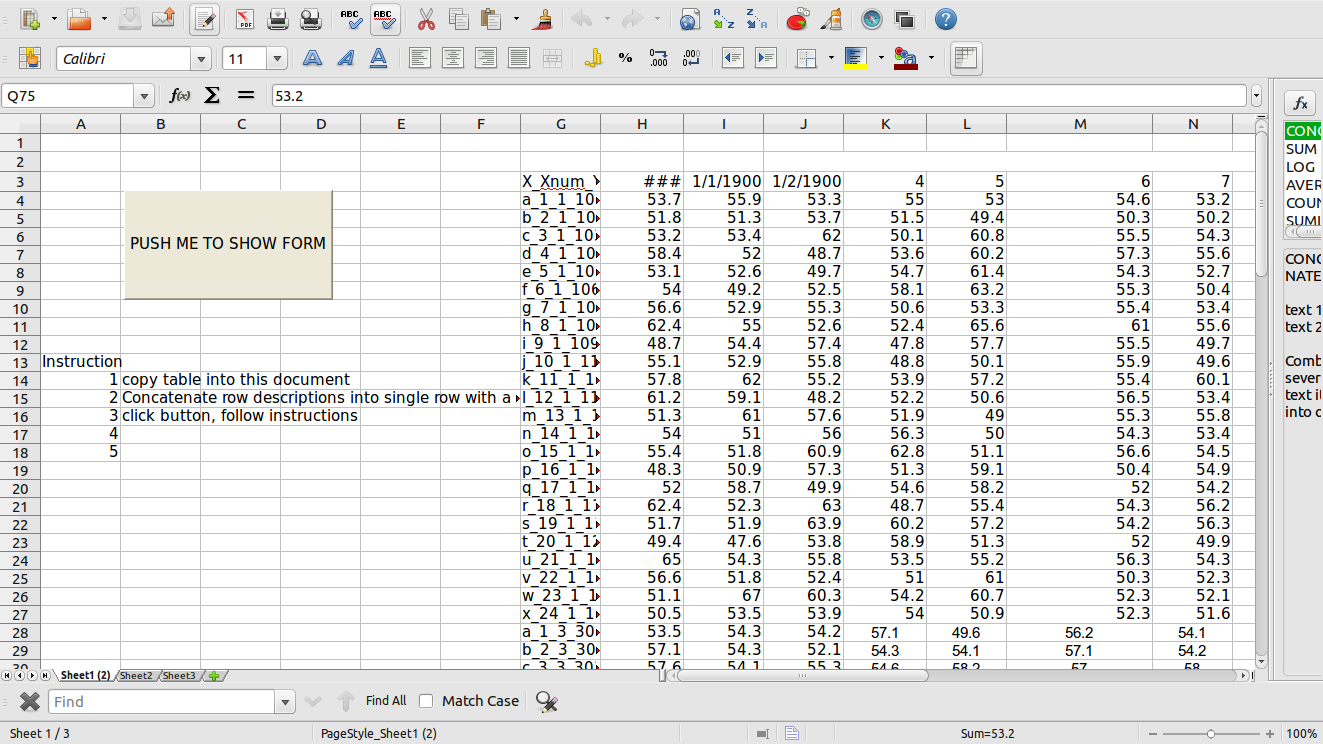
\includegraphics[width=.99\textwidth]{~/GitHub/FB/Ecoli_comparative_genomics/doc/presentations/MyNUIG(mnuigtheme)/20170303_ht_figs/macros.png}
\end{frame}

\begin{frame}[fragile]
  \frametitle{Bad Data}
  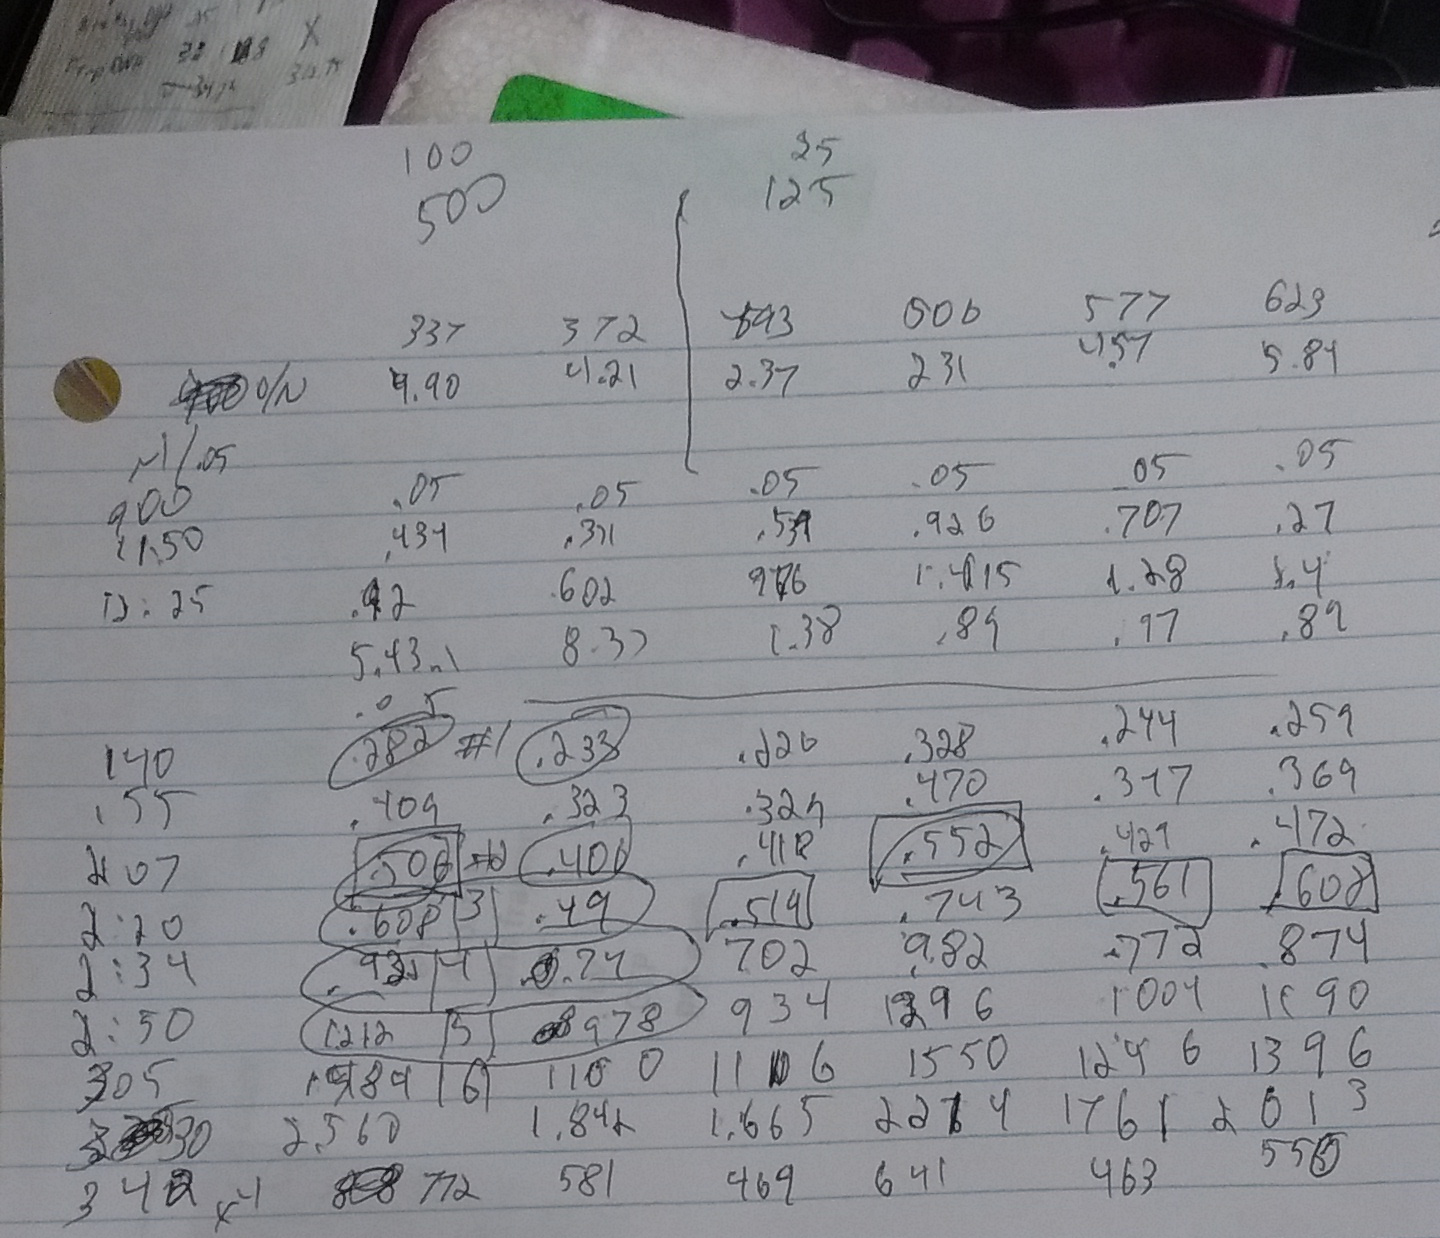
\includegraphics[width=.99\textwidth]{~/GitHub/FB/Ecoli_comparative_genomics/doc/presentations/MyNUIG(mnuigtheme)/20170303_ht_figs/IMG_20160204_160610788.jpg}
\end{frame}

\section{The Real Problem: Separation of Concerns}
\begin{frame}[fragile]
  \frametitle{Separation of Concerns}
  Separation of concerns: The practice of separating data from analysis.\\
  Why do we need to separate data from analysis?
  \begin{itemize}
  \item Saves time for repeated analysis
  \item Reproducible results
  \item Prevents data loss or contamination
  \item Prevents user error
  \item Easier to track over time
  \end{itemize}
\end{frame}

\begin{frame}[fragile]
  \frametitle{Data}
  Raw data should never be changed.

  \begin{itemize}
  \item Store it in plain text format in utf-8
  \item Store it with metadata in the same directory also in plain text
    \item Make sure it is backed up
  \end{itemize}
\end{frame}


\begin{frame}[fragile]
  \frametitle{Analysis with Excel}
  Do's:
  \begin{itemize}
  \item Include a ``metadata'' sheet
  \item Make new columns/rows for each step in analysis
  \item Document each step
  \item Explicitly set data types
  \end{itemize}
  Don'ts:
  \begin{itemize}
  \item Link Excel workbooks or sheets
  \item Rely on color coding
  \item Use macros
   \item Copy and paste
  \end{itemize}
\end{frame}

\begin{frame}[fragile]
  \frametitle{Analysis with Literate Programming}
  Literate programming mixes text description with data analysis.  Examples include Jupyter notebooks, knitr/sweave, emacs's org-mode.

  Do's:
  \begin{itemize}
  \item Explicitly state where the data is coming from
  \item Keep the analysis scoped to a single folder
  \item Document each step
    \item Ensure compilation will fail with ill-formatted data
  \item When finished, zip the entire directory for stable storage.
  \end{itemize}
  Don'ts:
  \begin{itemize}
  \item Mix literate programming with hardcoding
  \item Leave out print statements
  \item Forget sanity checks
  \end{itemize}
\end{frame}


\begin{frame}[fragile]
  \frametitle{Analysis with Code}
  R, python, MATLAB, etc

  Do's:
  \begin{itemize}
  \item Use version control
  \item Explicitly state where the data is coming from
  \item Write tests and comments for all the interesting steps
  \item Make the program write out a log
  \item Ensure compilation will fail with ill-formatted data
  \item Time-stamp results
  \end{itemize}
  Don'ts:
  \begin{itemize}
  \item Hard-code paths
  \item Write unhelpful comments
  \item Write similar code
  \item Forget sanity checks
  \item Rely on Stack Overflow
  \end{itemize}
\end{frame}

\section{Version control}

\begin{frame}[fragile]
  \frametitle{Overview}
  Version control keeps track of changes made to data and other files
  \begin{itemize}
  \item Dropbox/Google Drive
  \item Google docs
  \item Time Machine
    \item Lab wiki's
  \item Git, subversion, or murcurial
\end{itemize}
\end{frame}


\begin{frame}[fragile]
  \frametitle{Things that should be version controlled}
  \begin{itemize}
  \item Protocols
  \item Manuscripts
  \item Analysis pipeline
\end{itemize}
\end{frame}

\begin{frame}[fragile]
  \frametitle{Things that shouldn't be version controlled}
  \begin{itemize}
  \item Data: backups are different from version control
  \item Temporary files
  \item Complex file formats, big files, etc
\end{itemize}
\end{frame}

\section{Takeaways}
\begin{frame}[fragile]
  \frametitle{Moral of the Story}
  Write data for computers, write code for people
\end{frame}

\begin{frame}[fragile]
  \frametitle{Homework}
  \begin{itemize}
  \item Identify analyses that could be automated
  \item If you use excel, make a ``metadata'' sheet
  \item Never link Excel workbooks
  \item Restructure project folders
\end{itemize}
\end{frame}





% \plain{}{Questions?}

\end{document}
